% ----------------------------------------------------------
% Resultados
% ----------------------------------------------------------
\chapter{Análise dos Resultados}
\label{chap:result}
% ----------------------------------------------------------

Nesta seção serão analisados os resultados obtidos após a execução do algoritmo implementado. É importante reafirmar que devido às limitações de hardware e à complexidade do problema, o algoritmo deve ser executado por um período de tempo longo (dias ou até semanas), para se obter um agente com uma política ótima. Como a execução por esse período de tempo é inviável, a análise de sua eficiência é feita executando o mesmo por períodos de tempo menores e observando as melhoras de performance obtidas.

A \textbf{Figura \ref{fig:resultados_v1}} mostra os resultados obtidos de um modelo treinado durante cerca de 3150 episódios, sendo que os primeiros 556 episódios utilizaram uma política aleatória para coletar amostras para o \textit{buffer} de experiência. Os resultados são referentes aos episódios após o início do treinamento.

\begin{figure}[h]
  \centering
  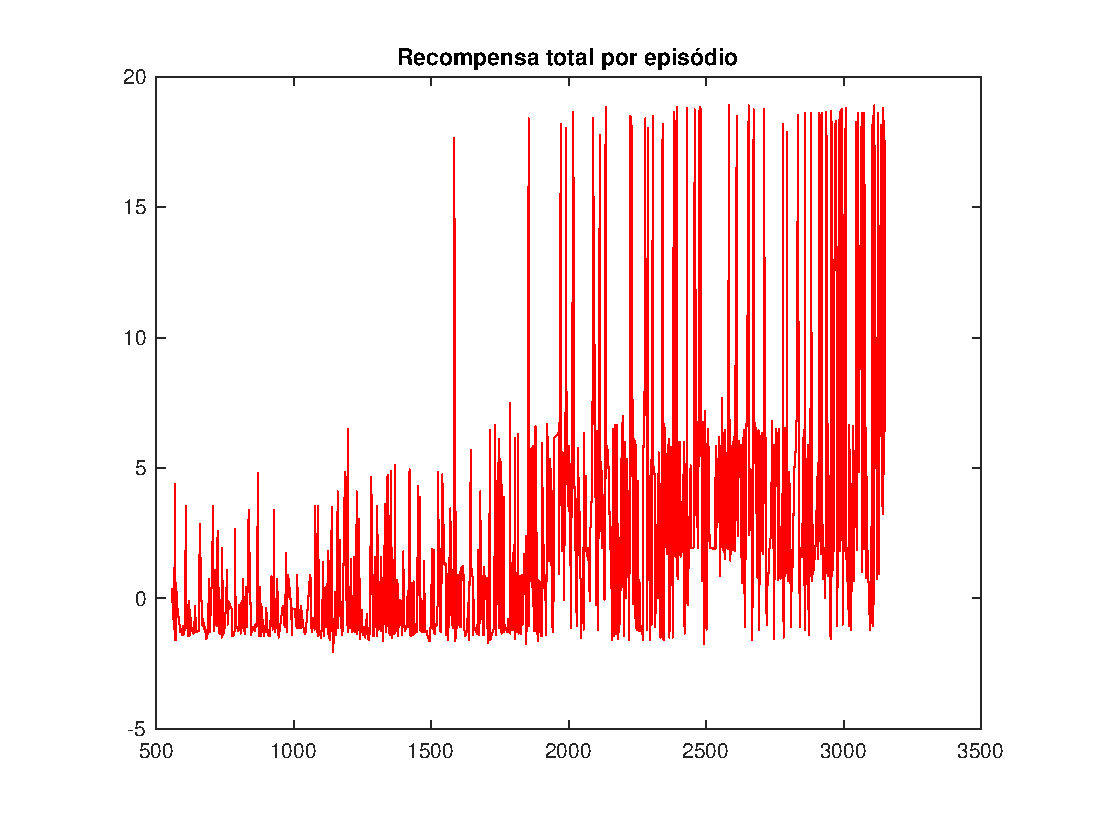
\includegraphics[width=.55 \textwidth]{conteudo/imgs/resultados/historico_recompensa_v1.eps}
  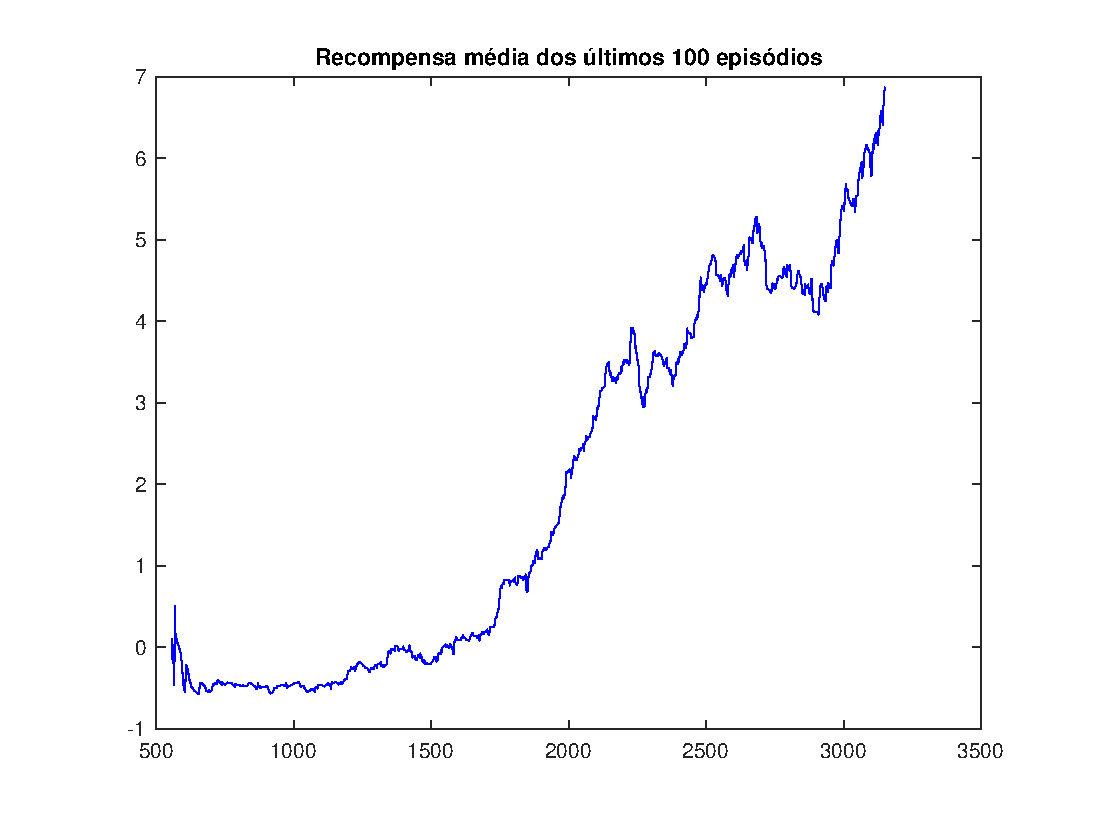
\includegraphics[width=.55 \textwidth]{conteudo/imgs/resultados/resompensa_media_100_epis_v1.eps}
  \caption[Resultados de Performance]{Resultados de um treinamento com 3150 episódios. A primeira imagem mostra as recompensas totais obtidas em cada episódio. A segunda indica a recompensa média dos 100 episódios anteriores}
  \label{fig:resultados_v1}
\end{figure}

De acordo com as recompensas estabelecidas na \textbf{Seção \ref{sub:o_jogo}}, a pontuação máxima possível a ser obtida por episódio é de $19pts$, sendo que qualquer pontuação $>10$ indica uma vitória do agente para aquele episódio. Além disso, qualquer pontuação $<2$ indica que o agente foi eliminado com pouco ou nenhum progresso no jogo.

Observando a \textbf{Figura \ref{fig:resultados_v1}}, podemos observar que a pontuação média dos primeiros 1500 episódios é negativa e próxima de zero, indicativos de uma política estocástica. Existem, mesmo nesse período inicial, alguns episódios no qual o agente foi capaz de obter algum progresso no jogo, mas no geral a sua performance foi ruim. Isso se dá ao fato de que, não somente a rede ainda não foi muito bem treinada, mas o valor de $\epsilon$ no início do treinamento é alto e próximo de 1, o que leva o agente a ter uma política próxima de uma política aleatória. 

Uma vez que o valor de $\epsilon$ começa a reduzir e a rede neural é treinada por um tempo considerável, os resultados começam a melhorar. O agente obtém sua primeira vitória no episódio 1584, e sua performance é aprimorada com o passar do tempo. Eventualmente, o algoritmo obtém vitórias consideravelmente mais frequentes e alcança uma pontuação média próxima de $7pts$ ao final dos 3150 episódios. Mesmo após esse treinamento, nota-se que o agente ainda não é capaz de vencer o jogo em boa parte dos episódios e ocasionalmente ainda obtém pontuações próximas de zero. Isso pode ser explicado pelo fato de que a rede precisa ser treinada por mais tempo e continuar aprimorando sua política. Além disso, o algoritmo utilizado tem o menor valor de $\epsilon_{min}=0.1$, isso faz que a qualquer momento, mesmo após o treinamento da rede, existe uma probabilidade de $10\%$ de que o agente irá tomar uma ação aleatória.

A \textbf{Figura \ref{fig:episodio2575}} mostra os quadros do episódio com a melhor pontuação obtida.

\begin{figure}[h]
  \centering
  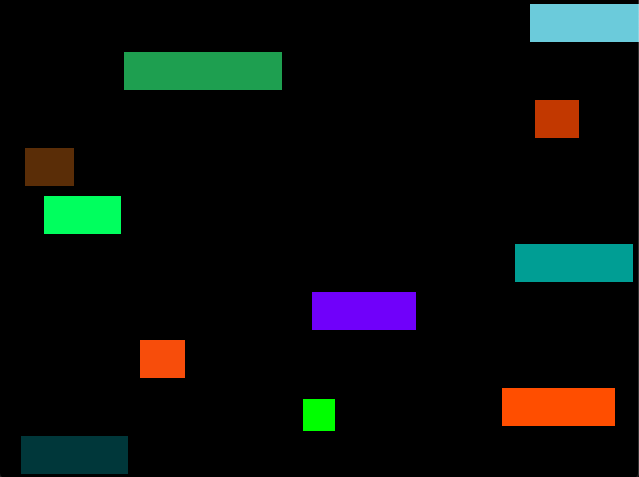
\includegraphics[width=.2 \textwidth]{conteudo/imgs/resultados/frogger_epi_1.png}
  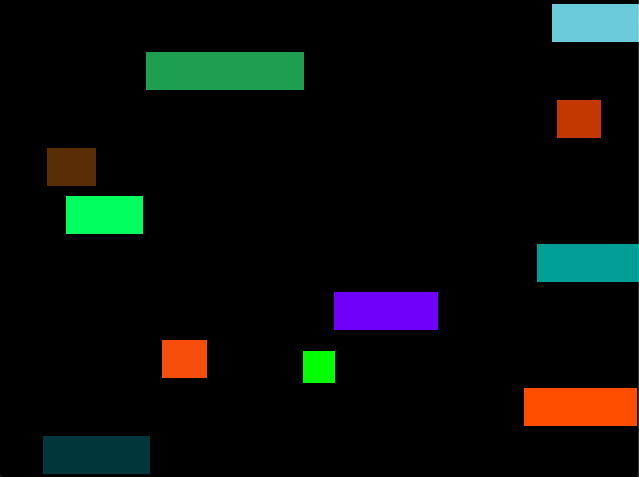
\includegraphics[width=.2 \textwidth]{conteudo/imgs/resultados/frogger_epi_2.png}
  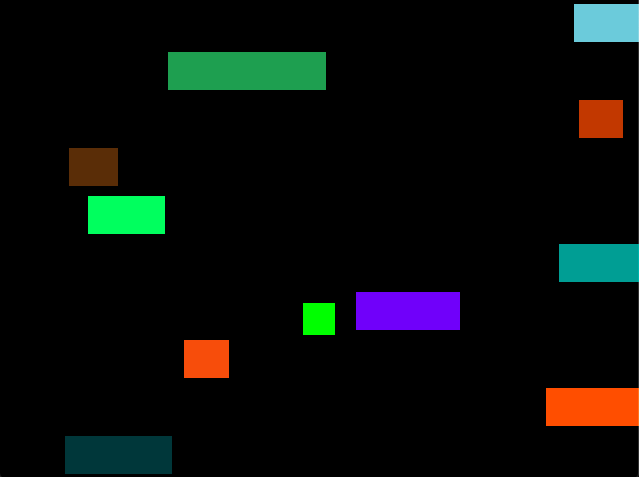
\includegraphics[width=.2 \textwidth]{conteudo/imgs/resultados/frogger_epi_3.png}
  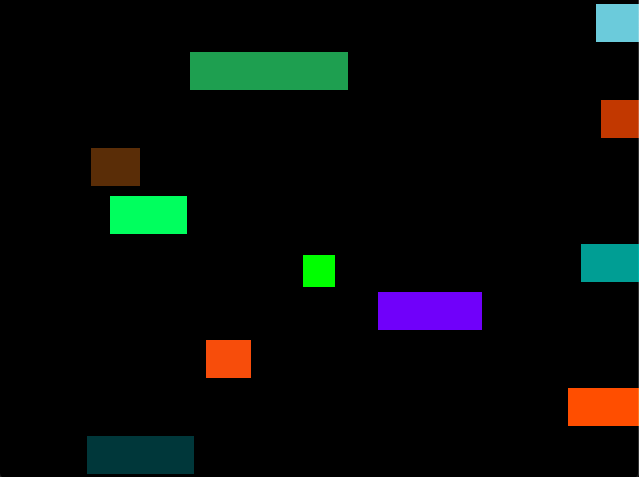
\includegraphics[width=.2 \textwidth]{conteudo/imgs/resultados/frogger_epi_4.png}
  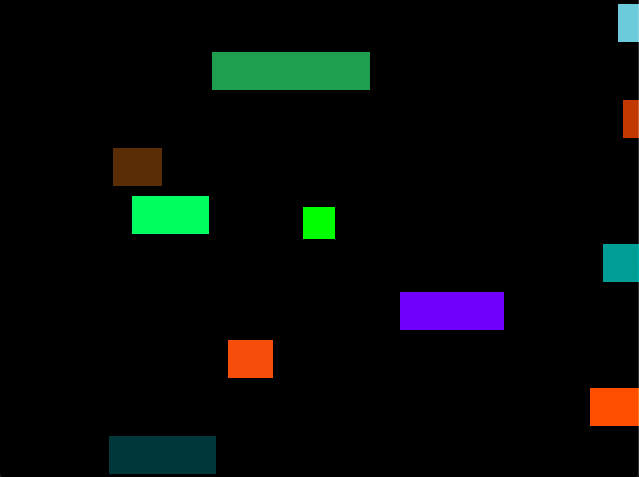
\includegraphics[width=.2 \textwidth]{conteudo/imgs/resultados/frogger_epi_5.png}
  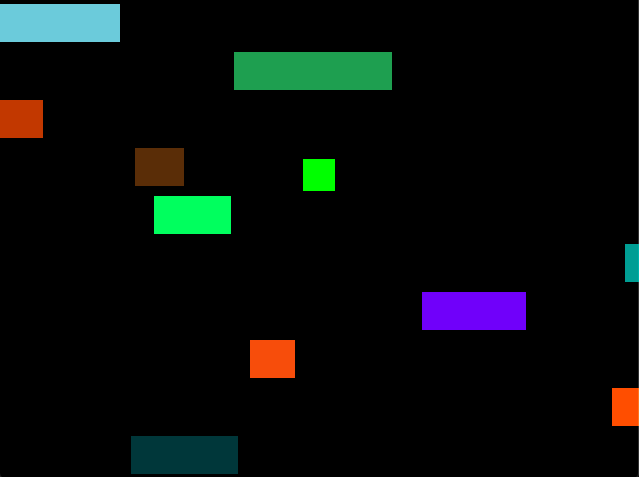
\includegraphics[width=.2 \textwidth]{conteudo/imgs/resultados/frogger_epi_6.png}
  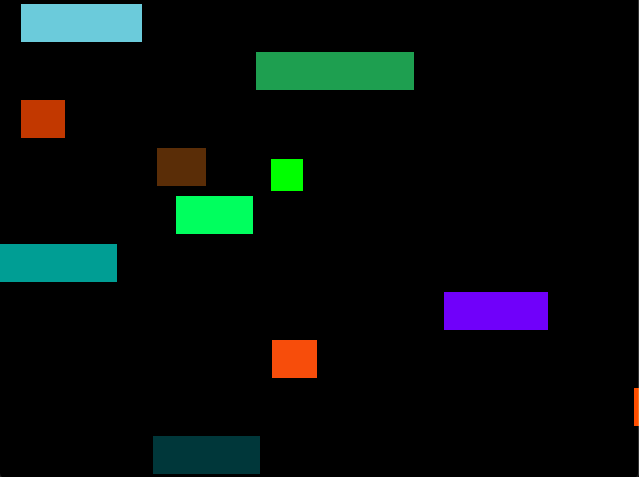
\includegraphics[width=.2 \textwidth]{conteudo/imgs/resultados/frogger_epi_7.png}
  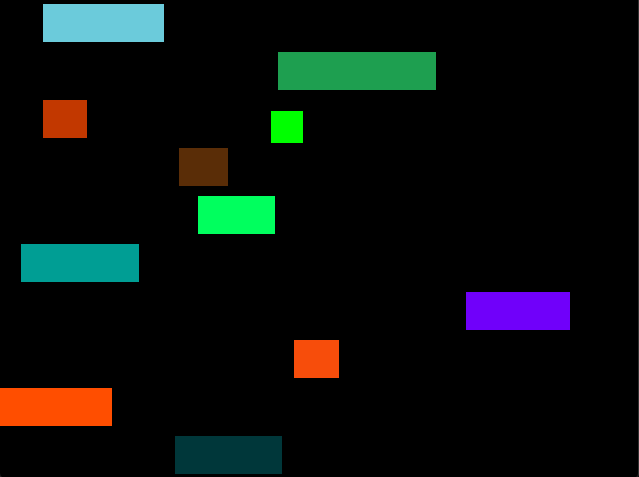
\includegraphics[width=.2 \textwidth]{conteudo/imgs/resultados/frogger_epi_8.png}
  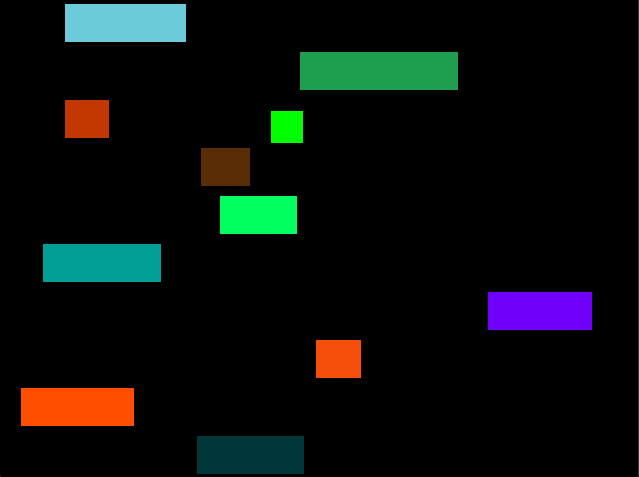
\includegraphics[width=.2 \textwidth]{conteudo/imgs/resultados/frogger_epi_9.png}
  
\includegraphics[width=.2 \textwidth]{conteudo/imgs/resultados/frogger_epi_10.png}
  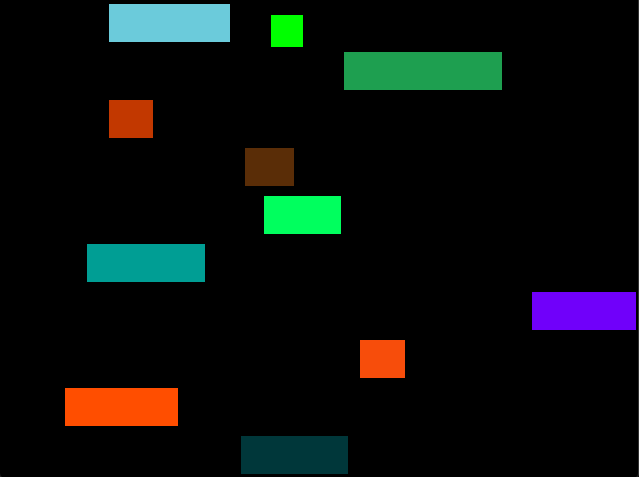
\includegraphics[width=.2 \textwidth]{conteudo/imgs/resultados/frogger_epi_11.png}
  
\includegraphics[width=.2 \textwidth]{conteudo/imgs/resultados/frogger_epi_12.png}
  \caption[Gameplay Episódio 2575]{Quadros do episodio 2575 onde o agente obteve uma pontuação de 18.9 pts}
  \label{fig:episodio2575}
\end{figure}

A \textbf{Figura \ref{fig:resultados_v2}} mostra os resultados de uma segunda rede treinada com diferentes parâmetros. É interessante notar que, mesmo a rede tendo sido treinada durante um número de episódios maior, a performance obtida não foi tão boa quanto a da primeira rede. Isso reflete a alteração dos valores dos parâmetros utilizados para essa iteração do algoritmo. Os principais parâmetros alterados foram o tamanho do \textit{buffer} de memória, o valor de $\epsilon$ e a frequência com o qual $\epsilon$ é atualizado.

\begin{figure}[h]
  \centering
  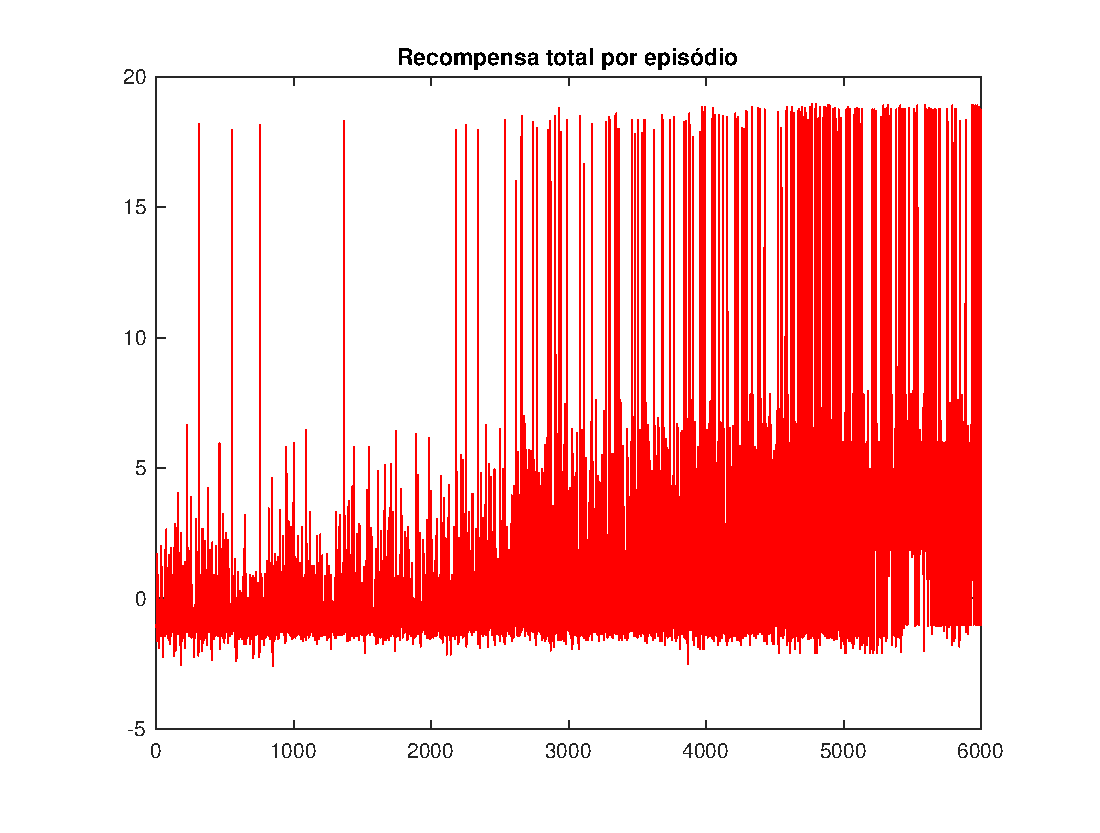
\includegraphics[width=.55 \textwidth]{conteudo/imgs/resultados/historico_recompensa_v2.eps}
  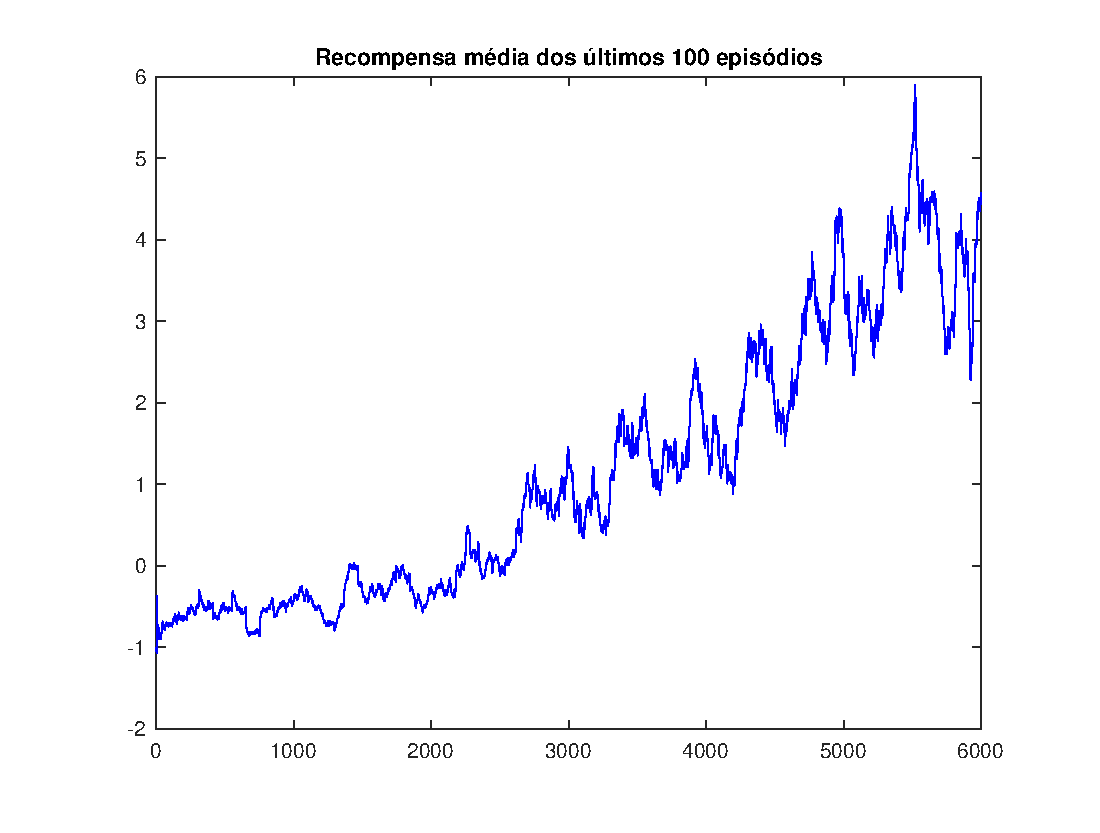
\includegraphics[width=.55 \textwidth]{conteudo/imgs/resultados/resompensa_media_100_epis_v2.eps}
  \caption[Resultados de Performance]{Resultados de um treinamento com 6000 episódios. A primeira imagem mostra as recompensas totais obtidas em cada episódio. A segunda indica a recompensa média dos 100 episódios anteriores}
  \label{fig:resultados_v2}
\end{figure}

O tamanho máximo do \textit{buffer} de memória foi aumentado em 10 vezes, enquanto o seu valor mínimo foi dobrado. Isso permite uma coleta maior de observações para treinamento da rede mas, em contrapartida, aumenta o número de episódios que serão executados antes de se iniciar o treinamento do agente. Além disso, o aumento do tamanho máximo do \textit{buffer} de memória faz com que a sobreposição dos dados do mesmo demore a ocorrer, tendo em vista que o \textit{buffer} irá armazenar 10 vezes mais dados antes de atingir seu volume máximo. Já o valor mínimo de $\epsilon$ foi definido com $\epsilon_{min}=0.05$, em vez de $\epsilon_{min}=0.1$, e o número de passos a serem dados, após o inicio do treinamento, para que $\epsilon$ varie de $1\rightarrow\epsilon_{min}$ foi de $20000$ da primeira rede, para $50000$ na segunda. Isso permite uma maior exploração do agente e por um período mais prolongado, mas aumenta o número de episódios necessários para que o agente reduza sua política estocástica.

Com isso, espera-se que a segunda rede obtenha melhores resultados a longo prazo, devido à sua maior exploração dos estados do jogo e maior quantidade e dados pra treinamento. No entanto, a curto prazo, a segunda rede deve demorar mais para alcançar bons resultados, o que explica os valores obtidos na \textbf{Figura \ref{fig:resultados_v2}}.
